\documentclass[a4paper]{article}
\usepackage[pdftex]{hyperref}
\usepackage[latin1]{inputenc}
\usepackage[english]{babel}
\usepackage{a4wide}
\usepackage{amsmath}
\usepackage{amssymb}
\usepackage{algorithmic}
\usepackage{algorithm}
\usepackage{ifthen}
\usepackage{listings}
\usepackage{array}
\usepackage{tabu}
% move the asterisk at the right position
\lstset{basicstyle=\ttfamily,tabsize=4,literate={*}{${}^*{}$}1}
%\lstset{language=C,basicstyle=\ttfamily}
\usepackage{moreverb}
\usepackage{palatino}
\usepackage{multicol}
\usepackage{tabularx}
\usepackage{comment}
\usepackage{verbatim}
\usepackage{color}
\usepackage{graphicx}
\usepackage{array,mathtools}
\usepackage{amsmath}

%% pdflatex?
\newif\ifpdf
\ifx\pdfoutput\undefined
\pdffalse % we are not running PDFLaTeX
\else
\pdfoutput=1 % we are running PDFLaTeX
\pdftrue
\fi
\ifpdf
\fi
\ifpdf
\DeclareGraphicsExtensions{.pdf, .jpg}
\else
\DeclareGraphicsExtensions{.eps, .jpg}
\fi

\parindent=0cm
\parskip=0cm

\setlength{\columnseprule}{0.4pt}
\addtolength{\columnsep}{2pt}

\addtolength{\textheight}{5.5cm}
\addtolength{\topmargin}{-26mm}
\pagestyle{empty}

%%
%% Sheet setup
%% 
\newcommand{\coursename}{Computer Architecture and Programming Languages}
\newcommand{\courseno}{CO20-320241}
\newcommand*{\carry}[1][1]{\overset{#1}}
\newcolumntype{B}[1]{r*{#1}{@{\,}r}}
 
\newcommand{\sheettitle}{Homework}
\newcommand{\mytitle}{}
\newcommand{\mytoday}{{14th of October}, 2019}

% Current Assignment number
\newcounter{assignmentno}
\setcounter{assignmentno}{5}

% Current Problem number, should always start at 1
\newcounter{problemno}
\setcounter{problemno}{1}

%%
%% problem and bonus environment
%%
\newcounter{probcalc}
\newcommand{\problem}[2]{
  \pagebreak[2]
  \setcounter{probcalc}{#2}
  ~\\
  {\large \textbf{Problem \textcolor{blue}{\arabic{assignmentno}}.\textcolor{blue}{\arabic{problemno}}} \hspace{0.2cm}\textit{#1}} \refstepcounter{problemno}\vspace{2pt}\\}

\newcommand{\bonus}[2]{
  \pagebreak[2]
  \setcounter{probcalc}{#2}
  ~\\
  {\large \textbf{Bonus Problem \textcolor{blue}{\arabic{assignmentno}}.\textcolor{blue}{\arabic{problemno}}} \hspace{0.2cm}\textit{#1}} \refstepcounter{problemno}\vspace{2pt}\\}

%% some counters  
\newcommand{\assignment}{\arabic{assignmentno}}

%% solution  
\newcommand{\solution}{\pagebreak[2]{\bf Solution:}\\}

%% Hyperref Setup
\hypersetup{pdftitle={Homework \assignment},
  pdfsubject={\coursename},
  pdfauthor={},
  pdfcreator={},
  pdfkeywords={Computer Architecture and Programming Languages},
  %  pdfpagemode={FullScreen},
  %colorlinks=true,
  %bookmarks=true,
  %hyperindex=true,
  bookmarksopen=false,
  bookmarksnumbered=true,
  breaklinks=true,
  %urlcolor=darkblue
  urlbordercolor={0 0 0.7}
}

\begin{document}


\coursename \hfill Course: \courseno\\
Jacobs University Bremen \hfill \mytoday\\
Fjolla Dedaj\hfill
\vspace*{0.3cm}\\
\begin{center}
{\Large \sheettitle{} \textcolor{blue}{\assignment}\\}
\end{center}


\problem{}{0}
\solution
\\
% expandable loop (used to avoid scope problems in tabular cells with the
% standard \loop)
\def\boucle #1\repeat {#1\b@@cle {#1}\repeat \repeat }
\def\b@@cle #1{\repeat #1\b@@cle {#1}}

\makeatletter
\newcount\@nn
\newcount\@mm
\newcount\@base
\newcount\@baseminusone

% please do not use this at home
% #1 must be a counter name, not something expanding to a number.
\def\@arabalpha #1{\ifcase #10\or1\or2\or3\or4\or5\or6\or7\or8\or9\or 
A\or B\or C\or D\or E\or F\or G\or H\or I\or J\or K\or L\or M\or N\or O\or
P\or Q\or R\or S\or T\or U\or V\or W\or X\or Y\or Z\fi}

\newcommand{\baseexpansion}[2][2]{% no negative numbers please!
\def\@digits{}%
\@base#1\relax \@baseminusone\@base\advance\@baseminusone-1
\@nn #2\relax  % this is the number to be written in base #1
%
\ifnum\@baseminusone<36
\def\onerow{#1\kern.1em\hbox{\vrule
   \vtop {\hbox{\ \the\@nn}\kern.3ex\hrule height.1ex }} &%
   \global\@mm\@nn \global\divide\@mm\@base 
   \multiply\@mm\@base \advance\@nn-\@mm 
   \the\@nn \xdef\@digits{\@arabalpha\@nn\@digits}}%
\else
\def\onerow{#1\kern.1em\hbox{\vrule
   \vtop {\hbox{\ \the\@nn}\kern.3ex\hrule height.1ex }} &%
   \global\@mm\@nn \global\divide\@mm\@base 
   \multiply\@mm\@base \advance\@nn-\@mm 
   \the\@nn \xdef\@digits{\the\@nn.\@digits}}%
\fi
%
\leavevmode\oalign{$#2_{10}:$\hfil\cr
      $\left.
      \begin{tabular}{r|l}
         \boucle \onerow \\ \ifnum\@nn>\@baseminusone\global\@nn\@mm \repeat
      \end{tabular}\right\rbrace=
      \mathtt{\@digits}_{#1}$}}     % \hfil removed from the macro

\makeatother

\lineskip12pt
\textbf{a)} $14 + 37 = 1110_2 + 100101_2 = 110011 $\\
\\
  \baseexpansion{14}\hfil
  \baseexpansion{37}\hfil
  \\
  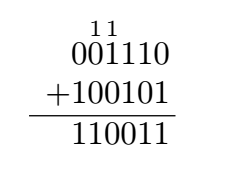
\includegraphics[scale=0.36]{1a.png}
  \\
\textbf{b)} $12 - 27 = 1110_2 + 100101_2 = 110001 $\\
\\
  \baseexpansion{12}\hfil
  \baseexpansion{27}\hfil
  \\
  Flip the bits and add 1 to get -27 (we need 6 bits in total to represent the sign also): $!(11011) + 1 = 00100 + 1 = 100101 $
  \\
  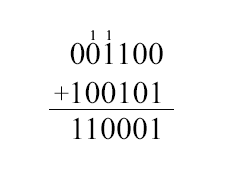
\includegraphics[scale=0.4]{1b.png}
  \\
\textbf{c)} $69 + 58 = 0110$ $1001 + 0101$ $0100 = 1$ $0010$ $0111 $\\
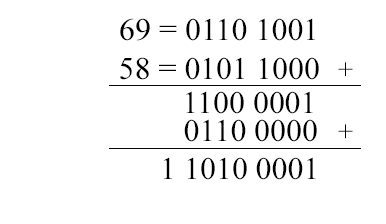
\includegraphics[scale=0.4]{1c.png}
\\
\textbf{d)} $ 275 + 642 = 100100010111$\\
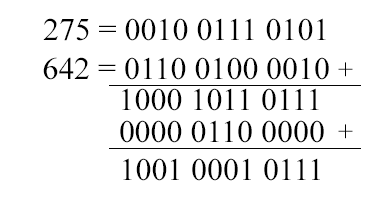
\includegraphics[scale=0.4]{1d.png}
\\
\pagebreak
\\
\textbf{e)} $6AF + 23C = 8EB$\\
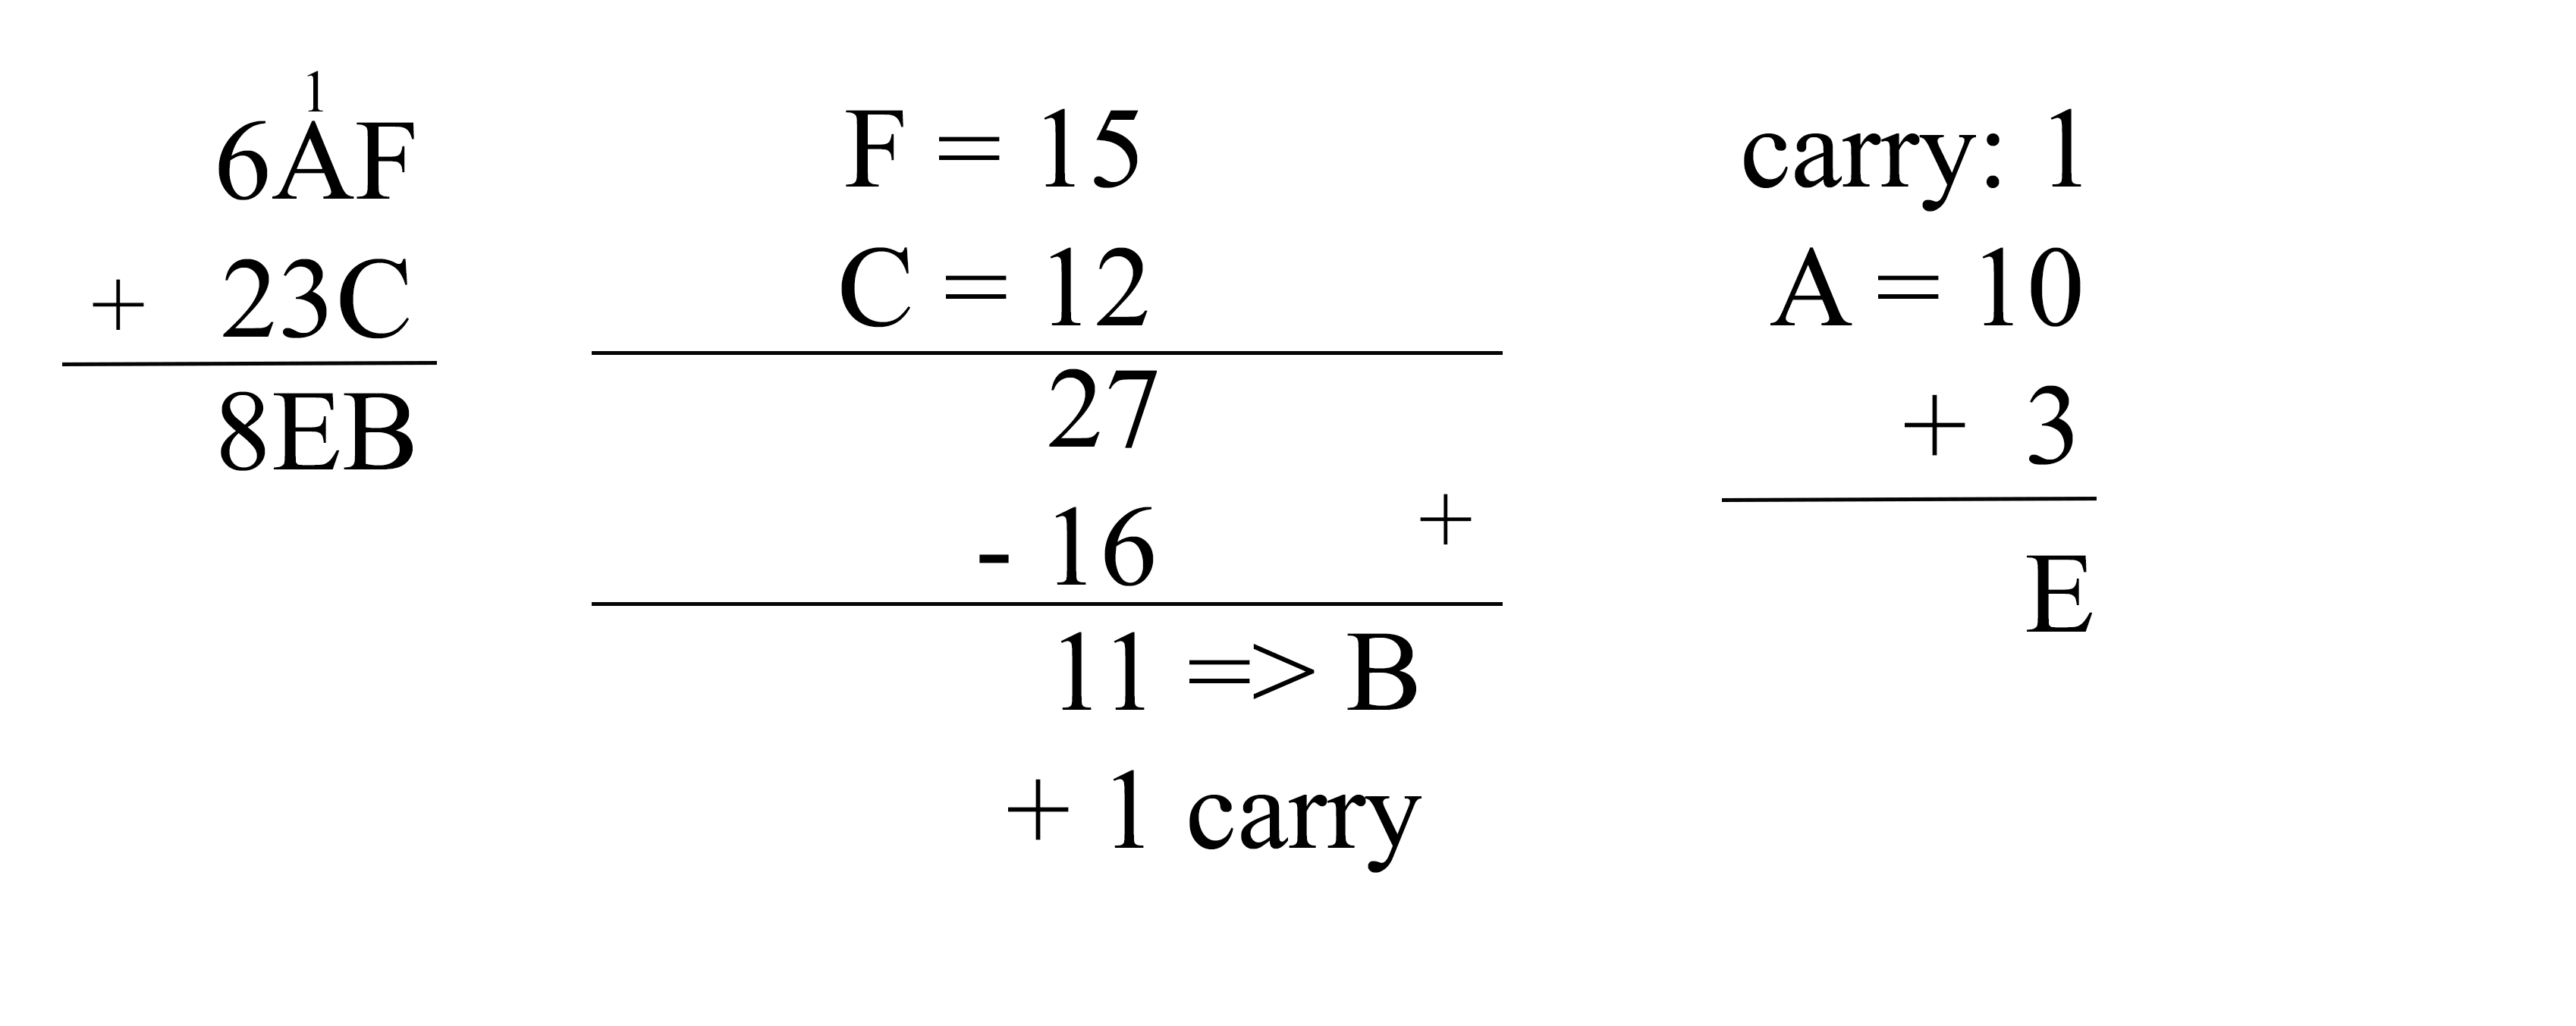
\includegraphics[scale=0.3]{1e.png}
\\
\textbf{f)} $594 - 3A8  = 1EC$\\
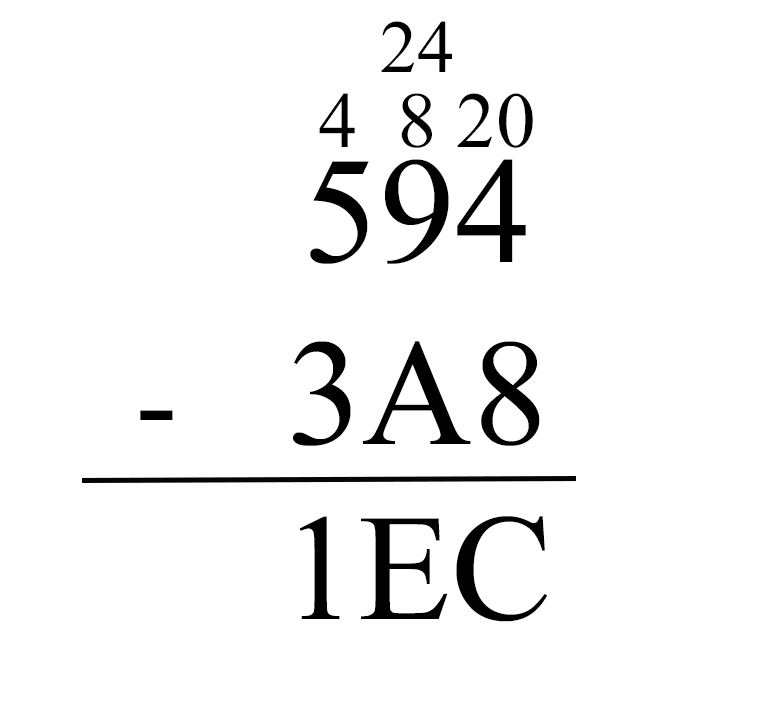
\includegraphics[scale=0.4]{1f.png}
\\
\problem{}{0}
\solution
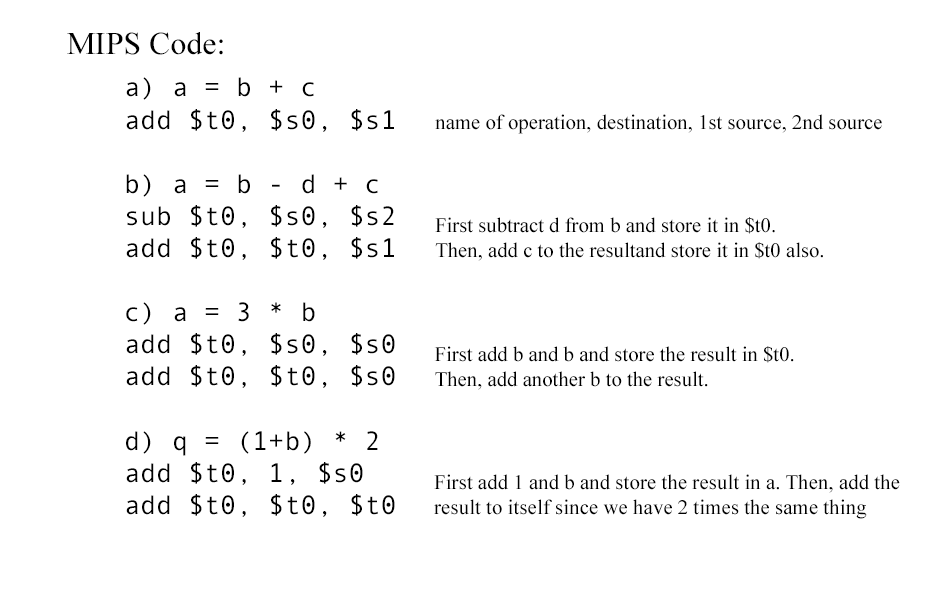
\includegraphics[scale=0.43]{problem2.png}
\problem{}{0}
\solution
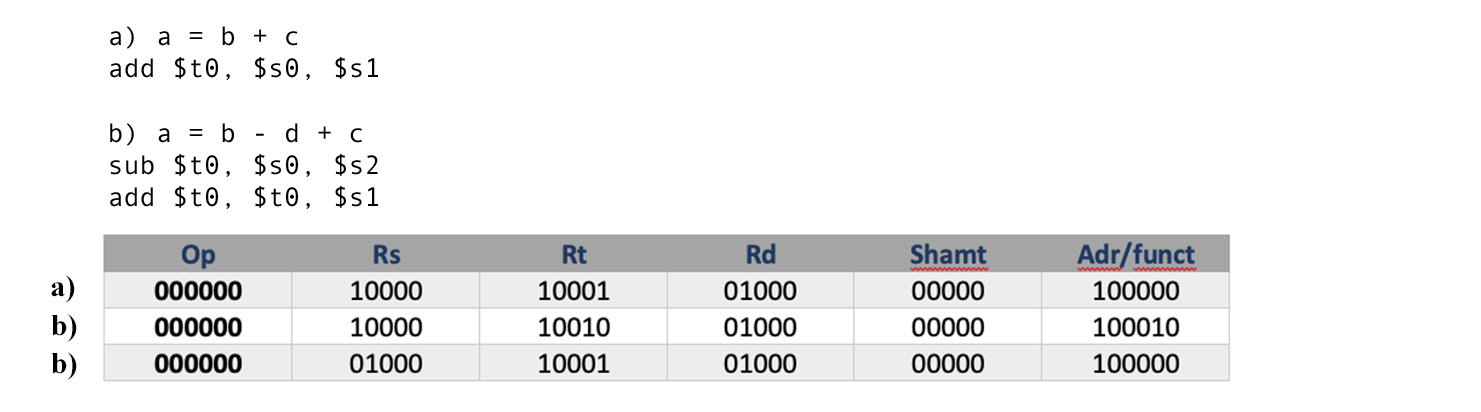
\includegraphics[scale=0.38]{problem3.png}
\\
\pagebreak
\\
\problem{}{0}
\solution
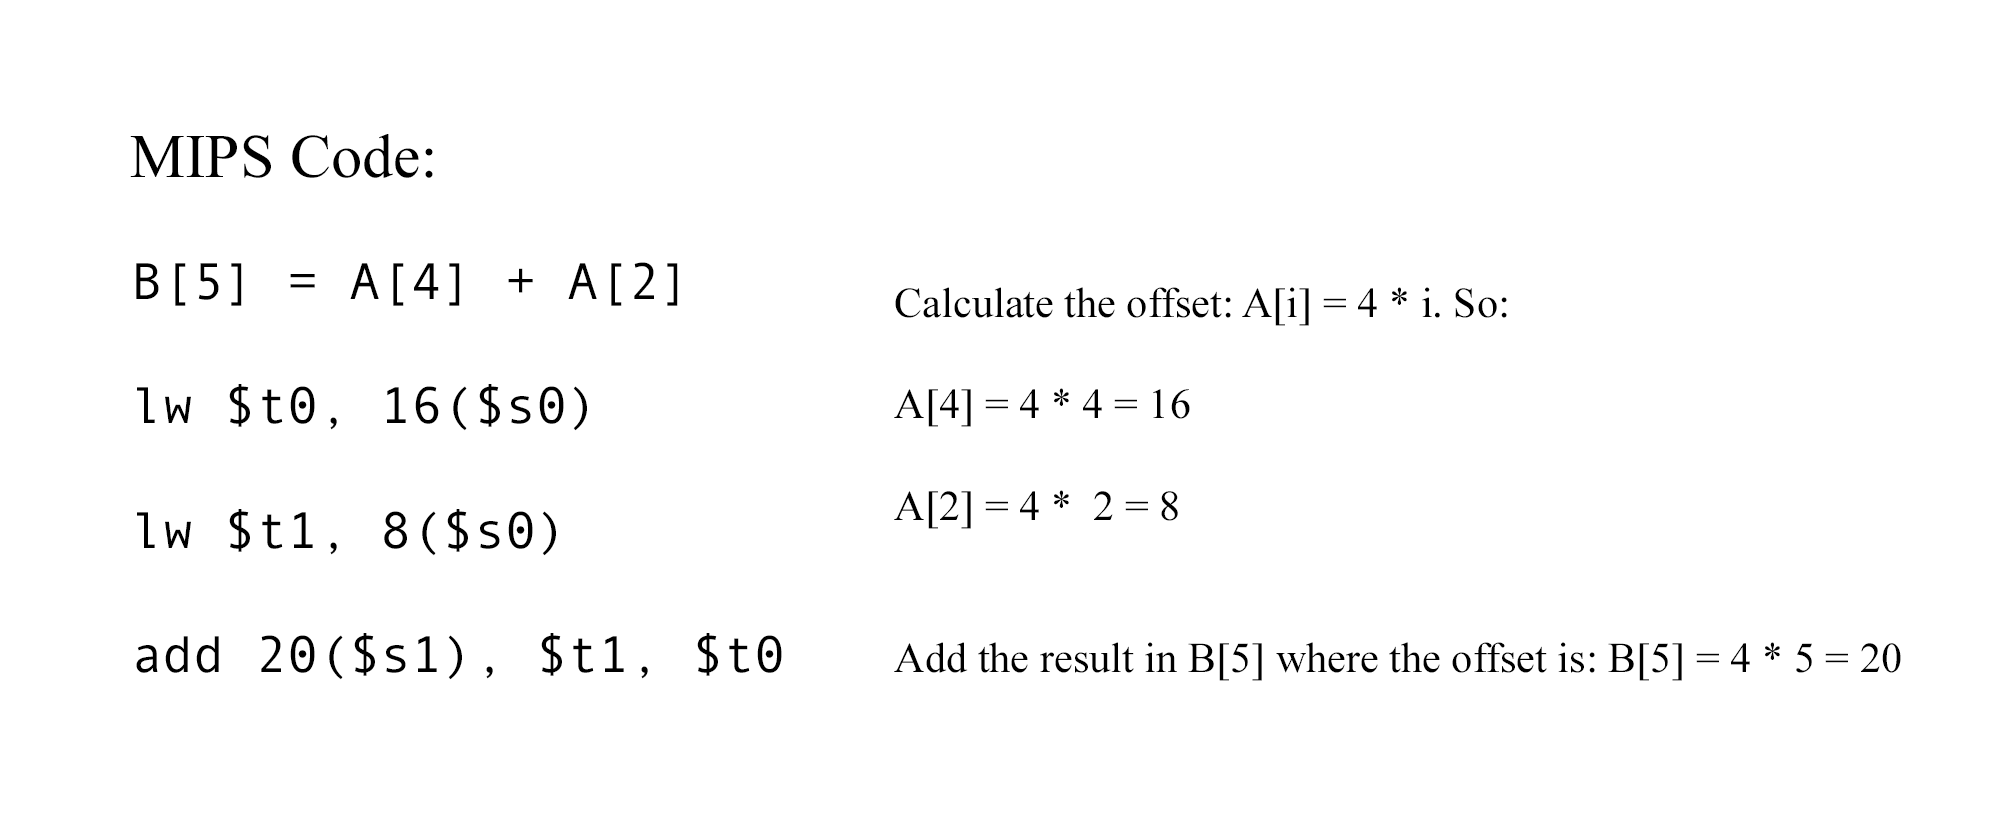
\includegraphics[scale=0.8]{problem4.png}
\problem{}{0}
\solution
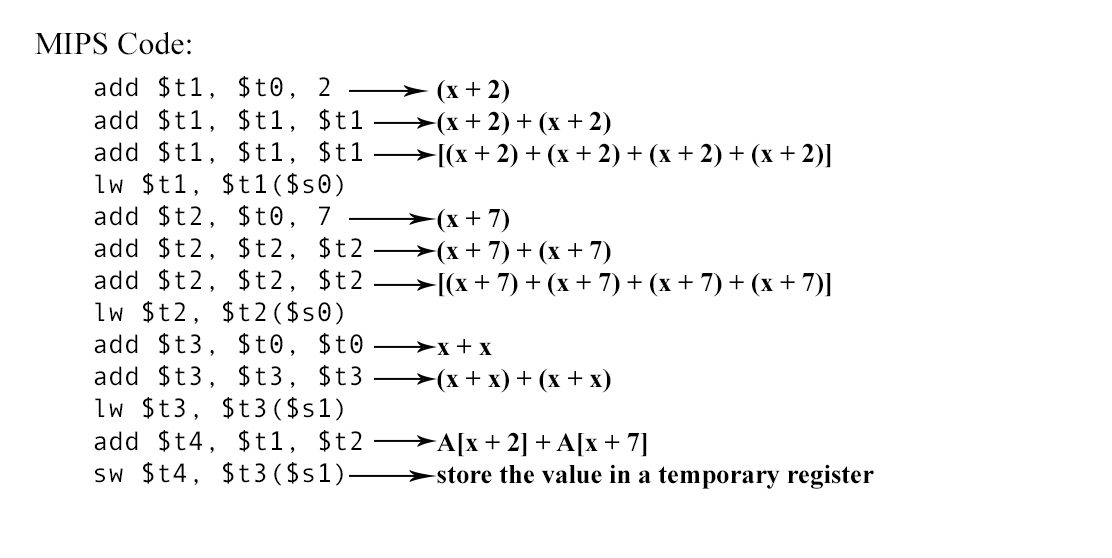
\includegraphics[scale=1.8]{problem5.png}
\\
\problem{}{0}
\solution\\
\textbf{The register instruction format for the instruction addi uses 6 bits for the opcode, 5 bits for the
first register, 5 bits for the second register, and 16 bits for the constant value that is to be added. Assume that a detailed analysis of machine code has revealed that not more than 12 registers are needed for the processor and therefore it has been decided to reduce the number of general purpose registers to 16. How and why could the instruction format for the addi instruction be changed?}\\
\\
\\
Addi copies the most significant bit (which is the sign bit) to all upper 16 bits of the destination. This is called sign extension. A negative operand would propagate 1's to the upper bits and watches for automatic sign extensions in arithmetic operations in MIPS. 16 higher bits of immediate operand are zeros, therefore it does the job.\\
\\
\\
To solve this assignment sheet, I collaborated with Dion Dermaku.
\end{document}